\documentclass[conference]{IEEEtran}
\IEEEoverridecommandlockouts

% ------------------------------ Core IEEE / citations ------------------------------
\usepackage{cite}

% ------------------------------ Math ------------------------------
\usepackage{amsmath,amssymb,amsfonts}

% ------------------------------ Figures / tables ------------------------------
\usepackage{graphicx}
\usepackage{textcomp}
\usepackage{xcolor}
\usepackage{multirow}

% ------------------------------ Links ------------------------------
\usepackage{hyperref}

% ------------------------------ Diagrams ------------------------------
\usepackage{tikz}
\usetikzlibrary{positioning,arrows.meta,fit,shapes.geometric}

% ------------------------------ Page style (optional) ------------------------------
\pagestyle{plain}

% ------------------------------ Commands ------------------------------
\newcommand{\R}{\mathbb{R}}
\newcommand{\E}{\mathbb{E}}
\newcommand{\W}{\mathsf{W}}
\newcommand{\KL}{\mathrm{KL}}
\newcommand{\pushfwd}{\sharp} % pushforward operator symbol for distributions

% ------------------------------ Title / authors ------------------------------
\title{
Learning Stage-to-Stage Cell State Transitions from Cross-Sectional Single-Cell Data via Optimal Transport Coupled Continuous Flows
\thanks{Course project topic proposal for EN.705.744 Deep Learning with Transformers, Johns Hopkins University.}
}

\author{
\IEEEauthorblockN{AJ Book}
\IEEEauthorblockA{
Johns Hopkins University \\
EN.705.744 Deep Learning with Transformers \\
Email: abook3@jhu.edu
}
}

\begin{document}

\maketitle

\begin{abstract}
Constructing predictive and mechanistic models of cellular state transitions is a central goal of modern single-cell biology and a prerequisite for credible virtual cell systems. Recent community efforts emphasize generalization across perturbations and contexts, as reflected by transformer models trained on hundreds of millions of cells and by emerging benchmarks that formalize evaluation as a Turing-like test for cellular prediction \cite{Roohani2025-yb,Adduri2025-nt,Dong2026-fb}. However, many biologically important transitions, including disease progression and tissue remodeling, are observed only through cross-sectional measurements rather than longitudinally tracked single cells, creating an identifiability bottleneck for learning state-to-state dynamics.

This proposal defines an applied machine learning problem that learns stage-to-stage transition operators between cell state distributions using cross-sectional single-cell data, and introduces a transformer-centered solution that couples optimal transport to continuous-time generative flows. The core modeling choice is a Set Transformer \cite{Lee2018-ya} that represents each stage as an unordered set of cells and learns permutation-invariant, context-aware embeddings that parameterize a continuous vector field governing a flow between stages. The training signal is constructed using entropically regularized optimal transport computed with Sinkhorn distances \cite{Cuturi2013-li}, which provides a principled distributional alignment prior \cite{Bunne2024-pl,Bunne2023-bm} and yields pseudo-pairings that enable flow matching objectives \cite{Lipman2022-ns} and Wasserstein-lifted variants \cite{Haviv2024-qe}. The project will deliver (i) formal hypotheses about when cross-sectional stage flows are learnable under transport-regularized constraints, (ii) a prototype implementation and ablations against established single-cell generative baselines \cite{Lopez2018-ns,Piran2024-ca}, and (iii) an evaluation plan that emphasizes out-of-context generalization and stage-transition fidelity, aligning with contemporary virtual cell goals \cite{Roohani2025-yb,Adduri2025-nt,Dong2026-fb}.
\end{abstract}

\section{Introduction and project goals}

Predicting how cells change state is a foundational scientific objective spanning development, disease progression, immune activation, and therapy response. In the last several years, the field has converged on the notion that scalable machine learning models should move beyond descriptive embeddings toward counterfactual or predictive models that can generalize across diverse contexts \cite{Szalata2024-jl}. This direction is reinforced by two recent trends. First, transformer models trained on atlas-scale single-cell corpora are increasingly evaluated by their capacity to generalize to unseen conditions and to perform context-dependent inference \cite{Adduri2025-nt,Dong2026-fb}. Second, the virtual cell framing motivates standardized evaluation datasets and metrics that explicitly reward predictive modeling of perturbation responses \cite{Roohani2025-yb}. These developments justify treating cell state transitions as an applied machine learning problem in which the goal is to infer transformations between distributions over cell states.

A major practical barrier is that many transition phenomena are not measured as paired trajectories of the same cell through time. Instead, datasets frequently provide cross-sectional snapshots of a tissue at discrete stages (for example, lesion grades, treatment phases, or disease states), sometimes with spatial profiling that reflects microenvironmental organization \cite{Peng2025-xu}. Even when longitudinal sampling exists at the patient level, single-cell measurements are destructive, and direct cell tracking is unavailable. Consequently, the learning task must be formulated as inferring a mapping between distributions of cell states rather than between paired cells.

The goal of this project is to learn a sequence of stage-to-stage transition operators from cross-sectional single-cell data, using an architecture that makes the transformer component essential rather than incidental. The proposed approach treats each stage as a set of observed cells and learns a permutation-invariant representation of that set using the Set Transformer \cite{Lee2018-ya}, which builds on attention mechanisms \cite{Vaswani2017-rb}. This set representation then parameterizes a continuous-time generative flow that transports the stage-$s$ distribution to the stage-$(s+1)$ distribution. Optimal transport provides an alignment prior that partially resolves the lack of pairings in cross-sectional data \cite{Bunne2024-pl,Bunne2023-bm}, while flow matching provides a scalable training objective for continuous normalizing flows without requiring reverse-time diffusion simulation \cite{Lipman2022-ns}. Recent work further suggests that bringing Wasserstein geometry directly into flow matching can be beneficial when the objects of interest are distributions or microenvironments rather than individual samples \cite{Haviv2024-qe,Haviv2025-kd}.

This proposal is intended for submission to the Human Cell Atlas General Meeting, where emphasis on generalization across tissues, conditions, and measurement technologies motivates methods that explicitly model cell sets, distribution shifts, and context dependence \cite{Tejada-Lapuerta2025-wz,Dong2026-fb,Adduri2025-nt}.

\section{Machine learning problem definition}

Let $\mathcal{X} \subset \R^G$ denote a representation space for single-cell profiles with $G$ measured features (for example, normalized gene expression). Consider a sequence of biological stages indexed by $s \in \{1,\dots,S\}$. For each stage $s$, a cross-sectional dataset provides an unordered set of observed cells
\[
X^{(s)} = \{x^{(s)}_i\}_{i=1}^{n_s}, \qquad x^{(s)}_i \in \mathcal{X},
\]
assumed to be sampled from an unknown distribution $P_s$ over $\mathcal{X}$. The applied machine learning objective is to learn a family of transition operators $\{T_{s \rightarrow s+1}\}_{s=1}^{S-1}$ such that the pushforward of $P_s$ under $T_{s \rightarrow s+1}$ approximates $P_{s+1}$:
\[
(T_{s \rightarrow s+1})_{\pushfwd} P_s \approx P_{s+1} \quad \text{for } s=1,\dots,S-1,
\]
while preserving biologically meaningful structure such as cell-type-conditioned relationships and stage-dependent covariates.

Two properties make this problem nontrivial and scientifically relevant. First, the mapping is underdetermined without additional inductive bias because infinitely many transports can map one distribution to another. Second, the biologically relevant notion of closeness between cells is not purely Euclidean and is sensitive to batch, platform, and covariate shifts, issues that have motivated probabilistic generative modeling in single-cell analysis \cite{Lopez2018-ns} and disentanglement-based approaches \cite{Piran2024-ca}. This proposal therefore couples two inductive biases: (i) optimal transport as a distributional alignment prior \cite{Bunne2024-pl,Cuturi2013-li}, and (ii) set-based transformers that model interactions within and across cell sets in a permutation-invariant manner \cite{Lee2018-ya}.

\section{Candidate solution: Set Transformer parameterized OT-coupled continuous flows}

\subsection{Set Transformer architecture and the attention mechanism}

The model uses a Set Transformer \cite{Lee2018-ya} to represent each stage as an unordered set of cells. Internally, it uses the scaled dot-product multi-head attention mechanism introduced in the Transformer \cite{Vaswani2017-rb}, arranged in permutation-equivariant and permutation-invariant blocks.

\subsubsection{Scaled dot-product attention}
Given queries $Q \in \R^{n \times d_k}$, keys $K \in \R^{m \times d_k}$, and values $V \in \R^{m \times d_v}$, attention is
\[
\mathrm{Attn}(Q,K,V)
=
\mathrm{softmax}\!\left(\frac{QK^\top}{\sqrt{d_k}}\right)V.
\]

\subsubsection{Multi-head attention}
With $h$ heads, each head computes attention in a learned subspace:
\[
\mathrm{head}_r
=
\mathrm{Attn}(QW_r^Q,\;KW_r^K,\;VW_r^V),
\quad r=1,\dots,h,
\]
and
\[
\mathrm{MHA}(Q,K,V)
=
\mathrm{Concat}(\mathrm{head}_1,\dots,\mathrm{head}_h)W^O.
\]

\subsubsection{Set Transformer blocks}
Let $X \in \R^{n \times d}$ be the matrix whose rows are cell embeddings in a stage (cells are the set elements). The Set Transformer uses:
\begin{itemize}
  \item \textbf{Self-Attention Block (SAB):} permutation-equivariant:
  \[
  \mathrm{SAB}(X) = \mathrm{LN}\!\big(X + \mathrm{MHA}(X,X,X)\big),
  \]
  followed by a position-wise feed-forward network with residual connection and layer normalization.
  \item \textbf{Induced Self-Attention Block (ISAB):} introduces $m$ learned inducing points $I \in \R^{m \times d}$:
  \[
  H = \mathrm{MHA}(I,X,X), \qquad
  \mathrm{ISAB}(X) = \mathrm{MHA}(X,H,H),
  \]
  followed by residual and feed-forward steps.
  \item \textbf{Pooling by Multi-head Attention (PMA):} produces a permutation-invariant summary using $k$ learned seed vectors $S \in \R^{k \times d}$:
  \[
  Z = \mathrm{MHA}(S,H,H).
  \]
\end{itemize}

In this project, PMA with $k=1$ yields a single stage context embedding:
\[
c_s = f_{\theta}(X^{(s)}) \in \R^d,
\]
which summarizes population composition and within-stage interactions relevant for predicting the transition.

\subsection{Conditional continuous-time flow parameterization}

Stage-to-stage dynamics are modeled by a conditional continuous normalizing flow defined by an ODE:
\[
\frac{d x(t)}{dt} = v_{\phi}\!\big(x(t), t, c_s\big), \qquad t \in [0,1],
\]
where $v_{\phi}$ is a neural vector field conditioned on the current state $x(t)$, time $t$, and the Set Transformer context $c_s$.

A minimal instantiation is an MLP that consumes a concatenated input $[x(t), \gamma(t), c_s]$, where $\gamma(t)$ is a time embedding (for example, sinusoidal). The initial prototype will keep $v_{\phi}$ simple so the Set Transformer remains the primary attention module and its contribution is directly testable.

Sampling proceeds by drawing $x(0) \sim P_s$ (empirical cells from stage $s$) and integrating the ODE to obtain $\tilde{x}(1)$, forming $\tilde{P}_{s+1}$.

\subsection{OT pseudo-pairings via Sinkhorn and the training loss}

Because cross-sectional data provide no true cell-to-cell correspondences, optimal transport defines soft pseudo-pairs between consecutive stages.

\subsubsection{Entropic OT (Sinkhorn)}
Given samples $\{x_i\}_{i=1}^{n}$ from stage $s$ and $\{y_j\}_{j=1}^{m}$ from stage $s+1$, define a cost matrix
\[
C_{ij} = c(x_i, y_j),
\]
where $c(\cdot,\cdot)$ is a chosen biological cost (initially squared Euclidean distance in a preprocessing embedding, with sensitivity analysis planned). The entropically regularized OT coupling is
\[
\pi^\star
=
\arg\min_{\pi \in U(a,b)}
\langle C,\pi\rangle
+
\varepsilon \sum_{i,j}\pi_{ij}(\log \pi_{ij}-1),
\]
where $U(a,b)$ enforces marginal constraints and $\varepsilon>0$ controls entropy \cite{Cuturi2013-li,Bunne2024-pl}.

\subsubsection{OT-informed probability paths}
Sample index pairs $(i,j)\sim \pi^\star$ and define an interpolation path:
\[
x_t = (1-t)x_i + t y_j, \qquad t \sim \mathrm{Unif}(0,1).
\]
The target velocity along this path is constant:
\[
u_t(x_t) = \frac{d x_t}{dt} = y_j - x_i.
\]

\subsubsection{Flow matching objective}
Flow matching regresses the model vector field toward the target velocity along OT-informed paths \cite{Lipman2022-ns}:
\[
\mathcal{L}_{\text{FM}}(\phi,\theta)
=
\E_{(i,j)\sim \pi^\star}\;
\E_{t \sim \mathrm{Unif}(0,1)}
\left[
\left\|
v_{\phi}(x_t, t, c_s)
-
(y_j - x_i)
\right\|_2^2
\right],
\]
with $c_s=f_{\theta}(X^{(s)})$ computed by the Set Transformer.

\subsubsection{Full training objective}
The prototype will minimize $\mathcal{L}_{\text{FM}}$. If needed, optional regularizers will be evaluated:
\[
\mathcal{L}
=
\mathcal{L}_{\text{FM}}
+
\lambda_{\text{ctx}}\mathcal{L}_{\text{ctx}}
+
\lambda_{\text{reg}}\mathcal{L}_{\text{reg}}.
\]
Here $\mathcal{L}_{\text{ctx}}$ can enforce context-consistent predictions across random subsamples of the same stage, and $\mathcal{L}_{\text{reg}}$ can include penalties such as weight decay or mild constraints on $v_{\phi}$.

\subsubsection{Connection to Wasserstein flow matching}
If time permits, the project will explore Wasserstein-lifted flow matching variants that treat contexts as distributions, aligning with the interpretation that the learning target is transport between distributions rather than pointwise pairing \cite{Haviv2024-qe,Haviv2025-kd}. This is an extension rather than a requirement for the core prototype.

\subsection{Block diagram of the proposed pipeline}

Figure~\ref{fig:block} provides a conceptual block diagram of the proposed method. The diagram is included because the grading rubric expects a block diagram in the method section, and because it clarifies how the Set Transformer, optimal transport, and flow matching interact.

\begin{figure}[t]
\centering
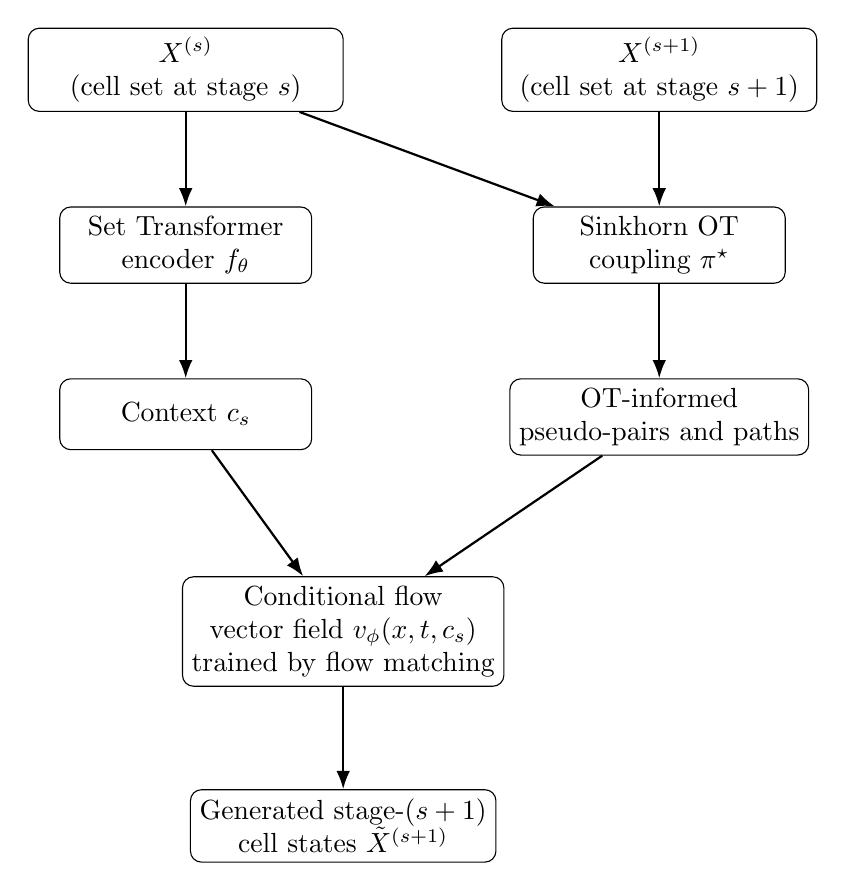
\begin{tikzpicture}[
  box/.style={draw, rounded corners, align=center, minimum width=4.0cm, minimum height=1.0cm},
  smallbox/.style={draw, rounded corners, align=center, minimum width=3.2cm, minimum height=0.9cm},
  arrow/.style={-Latex, thick}
]
\node[box] (xs) {$X^{(s)}$\\(cell set at stage $s$)};
\node[box, right=2.0cm of xs] (xt) {$X^{(s+1)}$\\(cell set at stage $s+1$)};

\node[smallbox, below=1.2cm of xs] (setenc) {Set Transformer\\encoder $f_{\theta}$};
\node[smallbox, below=1.2cm of xt] (ot) {Sinkhorn OT\\coupling $\pi^\star$};

\node[smallbox, below=1.2cm of setenc] (ctx) {Context $c_s$};
\node[smallbox, below=1.2cm of ot] (paths) {OT-informed\\pseudo-pairs and paths};

\node[box, below=1.6cm of ctx, xshift=2.0cm] (flow) {Conditional flow\\vector field $v_{\phi}(x,t,c_s)$\\trained by flow matching};

\node[smallbox, below=1.3cm of flow] (out) {Generated stage-$(s+1)$\\cell states $\tilde{X}^{(s+1)}$};

\draw[arrow] (xs) -- (setenc);
\draw[arrow] (setenc) -- (ctx);
\draw[arrow] (xs) -- (ot);
\draw[arrow] (xt) -- (ot);
\draw[arrow] (ot) -- (paths);
\draw[arrow] (ctx) -- (flow);
\draw[arrow] (paths) -- (flow);
\draw[arrow] (flow) -- (out);
\end{tikzpicture}
\caption{Block diagram of the proposed method. A Set Transformer encodes the source-stage cell set into a context vector, while Sinkhorn OT provides a coupling between consecutive stages. The coupling defines pseudo-pairings or OT-informed probability paths used to train a conditional continuous-time flow via flow matching.}
\label{fig:block}
\end{figure}

\section{Formal hypotheses}

This project tests whether stage-to-stage transitions inferred from cross-sectional data improve under (i) OT pseudo-pairings and (ii) Set Transformer context conditioning.

\subsection{Notation for evaluation metrics}

For each transition $s \rightarrow s+1$, let $\tilde{P}_{s+1}$ denote the model-generated distribution obtained by sampling $x \sim P_s$ and integrating the learned flow to time $t=1$. Let $\hat{P}_{s+1}$ be the empirical target distribution from held-out data at stage $s+1$.

Define a distributional discrepancy $D(\tilde{P}_{s+1}, \hat{P}_{s+1})$. In this project, $D$ will be instantiated as an entropically regularized OT (Sinkhorn) distance computed between generated and observed samples \cite{Cuturi2013-li}.

For generalization across biological contexts, let $\kappa$ index contexts (for example, donor, batch, or region). Let $\mathcal{K}_{\text{test}}$ be held-out contexts. Define the expected held-out discrepancy
\[
\mathcal{G}
=
\E_{\kappa \in \mathcal{K}_{\text{test}}}
\Big[
D\big(\tilde{P}_{s+1,\kappa}, \hat{P}_{s+1,\kappa}\big)
\Big].
\]

\subsection{Hypothesis 1: OT-coupled flow matching improves transition fidelity}

Let $\mathcal{M}_{\text{OT+FM}}$ be the proposed model trained with OT-derived pseudo-pairs and flow matching \cite{Lipman2022-ns,Bunne2023-bm}. Let $\mathcal{M}_{\text{noOT}}$ be an ablation that removes OT coupling (for example, uses random pairings or purely marginal matching).

Define
\[
\Delta_{\text{OT}}
=
D\big(\tilde{P}^{\text{OT+FM}}_{s+1}, \hat{P}_{s+1}\big)
-
D\big(\tilde{P}^{\text{noOT}}_{s+1}, \hat{P}_{s+1}\big).
\]

\textbf{Null hypothesis $H_0^{(1)}$:}
\[
H_0^{(1)}:\;\; \Delta_{\text{OT}} \ge 0.
\]

\textbf{Alternative hypothesis $H_1^{(1)}$:}
\[
H_1^{(1)}:\;\; \Delta_{\text{OT}} < 0.
\]

\subsection{Hypothesis 2: Set Transformer conditioning improves out-of-context generalization}

Let $\mathcal{M}_{\text{ctx}}$ be the proposed model with Set Transformer conditioning $c_{s,\kappa}=f_{\theta}(X^{(s)}_{\kappa})$ \cite{Lee2018-ya}. Let $\mathcal{M}_{\text{noctx}}$ be an ablation that removes context conditioning (the flow depends on $x,t$ only).

Define
\[
\Delta_{\text{ctx}}
=
\mathcal{G}_{\text{ctx}} - \mathcal{G}_{\text{noctx}},
\]
where
\[
\mathcal{G}_{\text{ctx}}
=
\E_{\kappa \in \mathcal{K}_{\text{test}}}
\Big[
D\big(\tilde{P}^{\text{ctx}}_{s+1,\kappa}, \hat{P}_{s+1,\kappa}\big)
\Big].
\]

\textbf{Null hypothesis $H_0^{(2)}$:}
\[
H_0^{(2)}:\;\; \Delta_{\text{ctx}} \ge 0.
\]

\textbf{Alternative hypothesis $H_1^{(2)}$:}
\[
H_1^{(2)}:\;\; \Delta_{\text{ctx}} < 0.
\]

\subsection{Optional secondary hypothesis: latent geometry improves interpolation fidelity}

If time permits, the project will evaluate whether enforcing a more Euclidean latent geometry improves interpolation and trajectory quality \cite{Palma2025-uk}. Let $\mathcal{M}_{\text{geom}}$ include a latent-geometry regularizer and $\mathcal{M}_{\text{base}}$ omit it. Define an interpolation error metric $E_{\text{interp}}$:
\[
H_0^{(3)}:\; E_{\text{interp}}(\mathcal{M}_{\text{geom}}) \ge E_{\text{interp}}(\mathcal{M}_{\text{base}}),
\]
\[
\qquad
H_1^{(3)}:\; E_{\text{interp}}(\mathcal{M}_{\text{geom}}) < E_{\text{interp}}(\mathcal{M}_{\text{base}}).
\]

\section{Related work and positioning}

Transformers have become the dominant architecture family for large-scale representation learning across modalities, and recent reviews argue that single-cell modeling is approaching a similar inflection point as atlas-scale datasets grow \cite{Szalata2024-jl}. The attention mechanism introduced in the original Transformer \cite{Vaswani2017-rb} supports flexible conditioning and long-range interactions, which can be repurposed to model sets of cells, neighborhoods, or gene programs. The Set Transformer is particularly relevant because it formalizes permutation invariance while retaining the representational advantages of attention \cite{Lee2018-ya}.

The virtual cell agenda emphasizes prediction across perturbations and contexts, motivating evaluation settings that test generalization \cite{Roohani2025-yb}. Large transformer systems trained on massive perturbed and observational datasets illustrate this direction, including models for predicting perturbation effects across diverse contexts \cite{Adduri2025-nt} and architectures that exploit tabular attention for in-context learning at the scale of hundreds of millions of cells \cite{Dong2026-fb}. Nicheformer represents a transformer trained to capture spatial context across dissociated and spatial modalities \cite{Tejada-Lapuerta2025-wz}, reinforcing the idea that population context and microenvironment structure should be explicit modeling targets.

Deep generative modeling has precedent in single-cell transcriptomics, including variational approaches that model technical noise and enable downstream tasks such as batch correction and differential expression \cite{Lopez2018-ns}. Disentanglement-oriented models such as biolord aim to separate known and unknown attributes and support counterfactual shifts across conditions \cite{Piran2024-ca}. Methods that impose topological templates, such as scPrisma, highlight mixing of biological programs and motivate structured inductive bias when reconstructing latent trajectories \cite{Karin2023-sa}. Recent work on hierarchical cross-entropy suggests that incorporating biological ontologies directly into learning objectives can improve out-of-distribution performance without increasing model complexity \cite{Cultrera-di-Montesano2026-vq}.

Optimal transport provides a framework for comparing and aligning distributions and is increasingly central in single-cell and spatial omics \cite{Bunne2024-pl}. Neural OT methods show that learning perturbation responses can be framed as transporting cell populations under unpaired observations, with gains in generalization \cite{Bunne2023-bm}. OT alone does not define a time-continuous generative model, and it can be expensive when repeated across many contexts. Transformer-based embedding approaches that approximate OT distances in Euclidean latent space address scalability and enable transport-aware operations such as barycenters and interpolations \cite{Haviv2024-uz}. Here, OT is used primarily as an alignment prior and supervision proxy, while the continuous dynamics model is learned via flow matching.

Flow matching defines a simulation-free objective for training continuous normalizing flows and supports probability paths defined by OT displacement interpolation \cite{Lipman2022-ns}. Wasserstein flow matching extends this by lifting flow matching onto families of distributions and using Wasserstein geometry to define valid conditional flows for generating distributions, including cellular microenvironments \cite{Haviv2024-qe}. This connects naturally to stage-to-stage learning, which is inherently about transporting distributions.

Spatial single-cell and spatial transcriptomics motivate methods that integrate dissociated and spatial modalities, including Tangram \cite{Biancalani2021-bt}, NovoSpaRc \cite{Moriel2021-wu}, cell2location \cite{Kleshchevnikov2022-ki}, and DestVI \cite{Lopez2022-ps}. Benchmarking studies emphasize that performance depends strongly on task definition, dataset properties, and evaluation metrics \cite{Li2022-uy}. Although this project will prioritize stage-to-stage transitions on cross-sectional scRNA-seq, these spatial methods motivate extensions in which transitions are learned jointly with niche context and provide downstream tests where inferred transitions can be interpreted in tissue organization settings. Deconvolution in tumor settings also highlights practical barriers from sparsity and compositional mixtures, motivating careful modeling choices and staged evaluation across sparsity regimes \cite{Montierth2025-ap}.

\section{Dataset plan and biological application context}

The project will use publicly available cross-sectional single-cell datasets that provide discrete stages corresponding to biological progression, treatment phase, or developmental time. A motivating application is lung tissue remodeling and lesion progression, where spatial and multimodal profiling has revealed stage-specific programs and epithelial-immune niches \cite{Peng2025-xu}. These transitions are typically observed as cross-sectional snapshots rather than longitudinally tracked single cells, providing a realistic setting where stage-to-stage transitions are biologically meaningful and plausibly depend on population composition and microenvironmental context.

The broader aim is a framework that can be evaluated on multiple stage-labeled datasets, including settings where spatial context or microenvironment composition is available, so the role of set-based context encoding can be tested against context-free baselines. Evaluation will prioritize avoiding trivial solutions that memorize stage labels and will emphasize held-out contexts (patients, donors, or experimental batches) to test generalization, consistent with virtual cell benchmarking \cite{Roohani2025-yb} and perturbation prediction across contexts \cite{Adduri2025-nt}.

\subsection{Primary datasets: early LUAD progression with spatial and single-nucleus profiling}

The primary empirical testbed will use two complementary GEO series from treatment-naive human lungs spanning a canonical sequence of pathogenesis: normal lung, atypical adenomatous hyperplasia (AAH), adenocarcinoma in situ (AIS), minimally invasive adenocarcinoma (MIA), and invasive LUAD. This staging structure matches the proposed learning objective, which is to infer transition operators between consecutive stage distributions.

\subsubsection{Spatial transcriptomics (Visium CytAssist; FFPE)}
GEO series \href{https://www.ncbi.nlm.nih.gov/geo/query/acc.cgi?acc=GSE307534}{GSE307534} contains 56 spatial transcriptomics samples generated with the 10x Genomics Visium CytAssist platform from surgically resected FFPE tissues. Several patients contribute paired lesions across stages, enabling within-patient evaluation and patient-held-out generalization tests. GEO notes that raw files for human samples were not submitted due to privacy concerns, but supplementary archives and processed outputs are available.

\subsubsection{Single-nucleus RNA-seq (10x Chromium Fixed RNA; FFPE)}
GEO series \href{https://www.ncbi.nlm.nih.gov/geo/query/acc.cgi?acc=GSE308103}{GSE308103} contains 75 snRNA-seq samples generated with the 10x Genomics Chromium Fixed RNA protocol on isolated nuclei from FFPE tissue scrolls. The stage structure mirrors the spatial series (normal, AAH, AIS, MIA, LUAD), and multiple patients contribute matched lesions, making it suitable for learning distributional flows while treating patient identity as a held-out context.

\subsection{Secondary benchmark: Virtual Cell Challenge datasets}

To align evaluation with contemporary virtual cell criteria and to test generalization in a community-facing benchmark setting, the project will optionally evaluate on datasets curated by the Virtual Cell Challenge (\href{https://virtualcellchallenge.org/datasets}{virtualcellchallenge.org/datasets}) associated with \cite{Roohani2025-yb}. These datasets reward predictive modeling under distribution shift. They serve as a complementary benchmark to stress-test out-of-context generalization and distributional fidelity, with conditions treated analogously to discrete stages when appropriate.

\section{Evaluation plan and performance criteria}

Evaluation will quantify whether learned transition operators produce stage-$(s+1)$ distributions that match empirical data while preserving meaningful biological structure. Primary criteria include distributional fidelity measured by Sinkhorn-approximated Wasserstein distances between generated and observed distributions \cite{Cuturi2013-li}, complemented by discrepancies such as MMD or classifier two-sample tests. Because OT distances can be expensive at evaluation time, transformer-based embeddings that approximate OT geometry will be explored as diagnostics and potentially as an auxiliary objective \cite{Haviv2024-uz}.

Biological plausibility will be assessed through gene program analyses. Stage transitions should recapitulate known stage-associated programs and differential expression patterns while preserving cell-type-conditioned structure rather than collapsing distinct populations. Where ontology labels are available, hierarchical evaluation will be considered to test whether errors respect biological hierarchies \cite{Cultrera-di-Montesano2026-vq}. Comparisons will include representative baselines: variational generative models \cite{Lopez2018-ns}, disentanglement-based counterfactual models \cite{Piran2024-ca}, and OT-based perturbation modeling \cite{Bunne2023-bm}. Ablations will isolate the effects of Set Transformer conditioning and OT-derived pseudo-pairings.

\section{Feasibility, limitations, and anticipated risks}

A central scientific risk is identifiability. Cross-sectional snapshots do not uniquely determine individual trajectories, and without constraints the model may learn transports that match marginals while violating plausible continuity. Optimal transport imposes a minimum-cost alignment, but the cost function can encode bias, and entropic regularization trades sharpness for stability \cite{Cuturi2013-li}. This project treats OT as a prior rather than as ground truth and will test sensitivity to cost choice and regularization strength.

A second risk is confounding by batch and technical effects. Probabilistic approaches such as scVI show that modeling technical variation can materially affect inference \cite{Lopez2018-ns}. The project will mitigate this by standard preprocessing and, where appropriate, training on latent embeddings rather than raw counts, while acknowledging that incorrect normalization can create spurious transitions.

A third risk is that stage labels may be coarse proxies for continuous progression. The model may be penalized for predicting heterogeneity that exists within a stage. This motivates diagnostics examining whether inferred flows preserve within-stage variation and whether trajectories align with interpretable axes, including geometry-regularized latent spaces \cite{Palma2025-uk} and topological signal decoupling approaches \cite{Karin2023-sa}.

\section{Expected outcomes and significance}

If successful, the project will produce a transformer-centered prototype for learning stage-to-stage transitions when only cross-sectional single-cell data are available. The key idea is to treat each stage as a set-level object, learn stage context via a Set Transformer \cite{Lee2018-ya}, and couple OT-based alignment \cite{Bunne2024-pl,Cuturi2013-li} with continuous-time generative modeling via flow matching \cite{Lipman2022-ns}. This aligns with trends emphasizing context-aware generalization and evaluation frameworks for virtual cells \cite{Roohani2025-yb,Adduri2025-nt,Dong2026-fb}. Longer-term relevance to the Human Cell Atlas community is that a distributional, context-conditioned approach can complement atlas efforts that integrate dissociated and spatial modalities \cite{Tejada-Lapuerta2025-wz,Biancalani2021-bt,Kleshchevnikov2022-ki,Lopez2022-ps,Moriel2021-wu}.

\bibliographystyle{IEEEtran}
\bibliography{references}

\end{document}
